%%%%%%%%%%%%%%%%%%%%%%%%%%%%%%%%%%%%%%%%%
% Beamer Presentation
% LaTeX Template
% Version 1.0 (10/11/12)
%
% This template has been downloaded from:
% http://www.LaTeXTemplates.com
%
% License:
% CC BY-NC-SA 3.0 (http://creativecommons.org/licenses/by-nc-sa/3.0/)
%
%%%%%%%%%%%%%%%%%%%%%%%%%%%%%%%%%%%%%%%%%

%----------------------------------------------------------------------------------------
%	PACKAGES AND THEMES
%----------------------------------------------------------------------------------------

\documentclass{beamer}

\mode<presentation> {

% The Beamer class comes with a number of default slide themes
% which change the colors and layouts of slides. Below this is a list
% of all the themes, uncomment each in turn to see what they look like.

%\usetheme{default}
%\usetheme{AnnArbor}
%\usetheme{Antibes}
%\usetheme{Bergen}
%\usetheme{Berkeley}
%\usetheme{Berlin}
%\usetheme{Boadilla}
%\usetheme{CambridgeUS}
%\usetheme{Copenhagen}
%\usetheme{Darmstadt}
%\usetheme{Dresden}
%\usetheme{Frankfurt}
%\usetheme{Goettingen}
%\usetheme{Hannover}
%\usetheme{Ilmenau}
%\usetheme{JuanLesPins}
%\usetheme{Luebeck}
\usetheme{Madrid}
%\usetheme{Malmoe}
%\usetheme{Marburg}
%\usetheme{Montpellier}
%\usetheme{PaloAlto}
%\usetheme{Pittsburgh}
%\usetheme{Rochester}
%\usetheme{Singapore}
%\usetheme{Szeged}
%\usetheme{Warsaw}

% As well as themes, the Beamer class has a number of color themes
% for any slide theme. Uncomment each of these in turn to see how it
% changes the colors of your current slide theme.

%\usecolortheme{albatross}
%\usecolortheme{beaver}
%\usecolortheme{beetle}
%\usecolortheme{crane}
%\usecolortheme{dolphin}
%\usecolortheme{dove}
%\usecolortheme{fly}
%\usecolortheme{lily}
%\usecolortheme{orchid}
%\usecolortheme{rose}
%\usecolortheme{seagull}
%\usecolortheme{seahorse}
%\usecolortheme{whale}
%\usecolortheme{wolverine}

%\setbeamertemplate{footline} % To remove the footer line in all slides uncomment this line
%\setbeamertemplate{footline}[page number] % To replace the footer line in all slides with a simple slide count uncomment this line

%\setbeamertemplate{navigation symbols}{} % To remove the navigation symbols from the bottom of all slides uncomment this line
}

\usepackage{graphicx} 
\usepackage{booktabs} 
\usepackage{hyperref}
\usepackage{amsmath}
\usepackage{epstopdf}

%----------------------------------------------------------------------------------------
%	TITLE PAGE
%----------------------------------------------------------------------------------------

\title[Introduction]{Positive and negative feedback}

\author{Slides courtesy of prof. Rodolphe Sepulchre}
\date{\today}

\begin{document}

\begin{frame}
\titlepage
\end{frame}

%----------------------------------------------------------------------------------------
%	PRESENTATION SLIDES
%----------------------------------------------------------------------------------------

\begin{frame}
\frametitle{Range-localized sensitivity is a nonlinear behavior}
\center{\Large{$V = sat(I)$}}
\begin{figure}
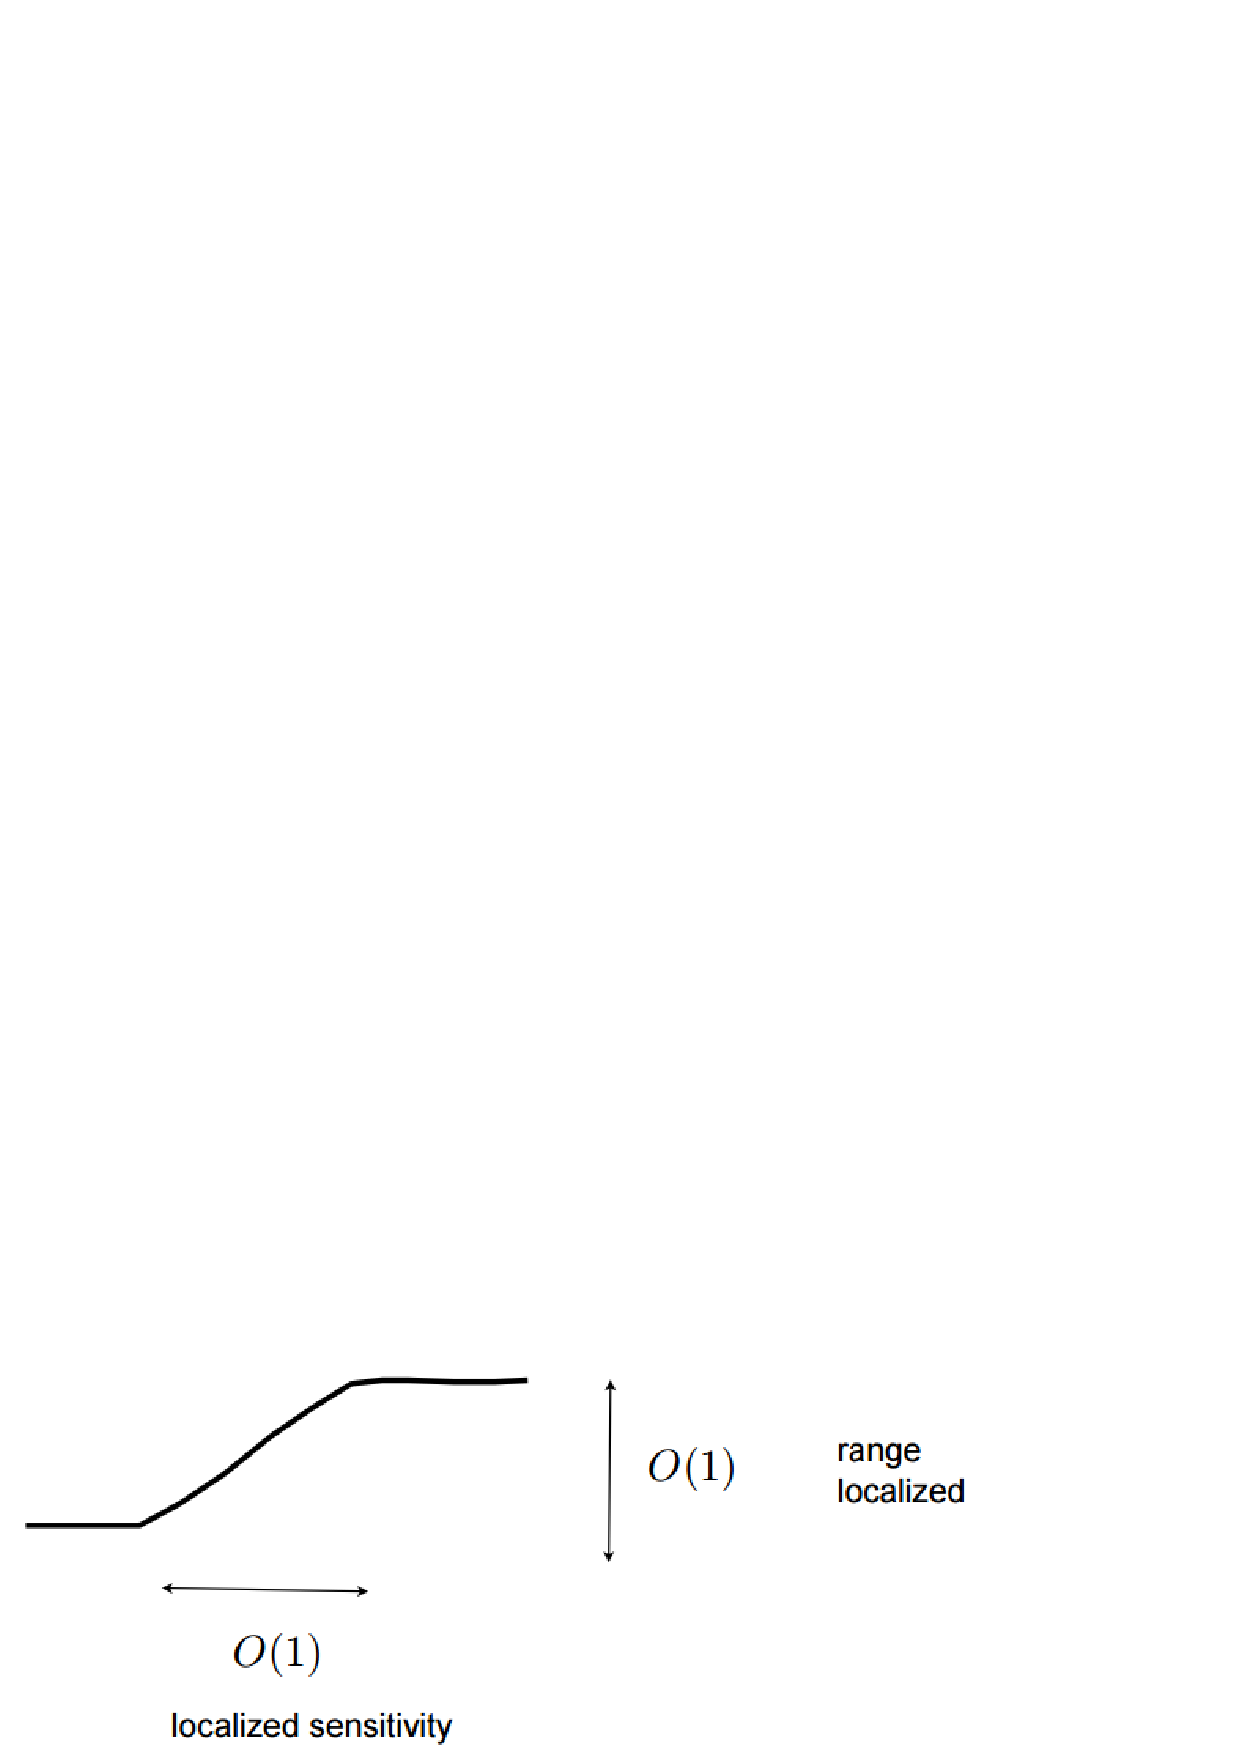
\includegraphics[width=1\linewidth]{range_localization}
\end{figure}
\end{frame}

%------------------------------------------------

\begin{frame}
\frametitle{Black principle: negative feedback 'linearizes'}
\begin{figure}
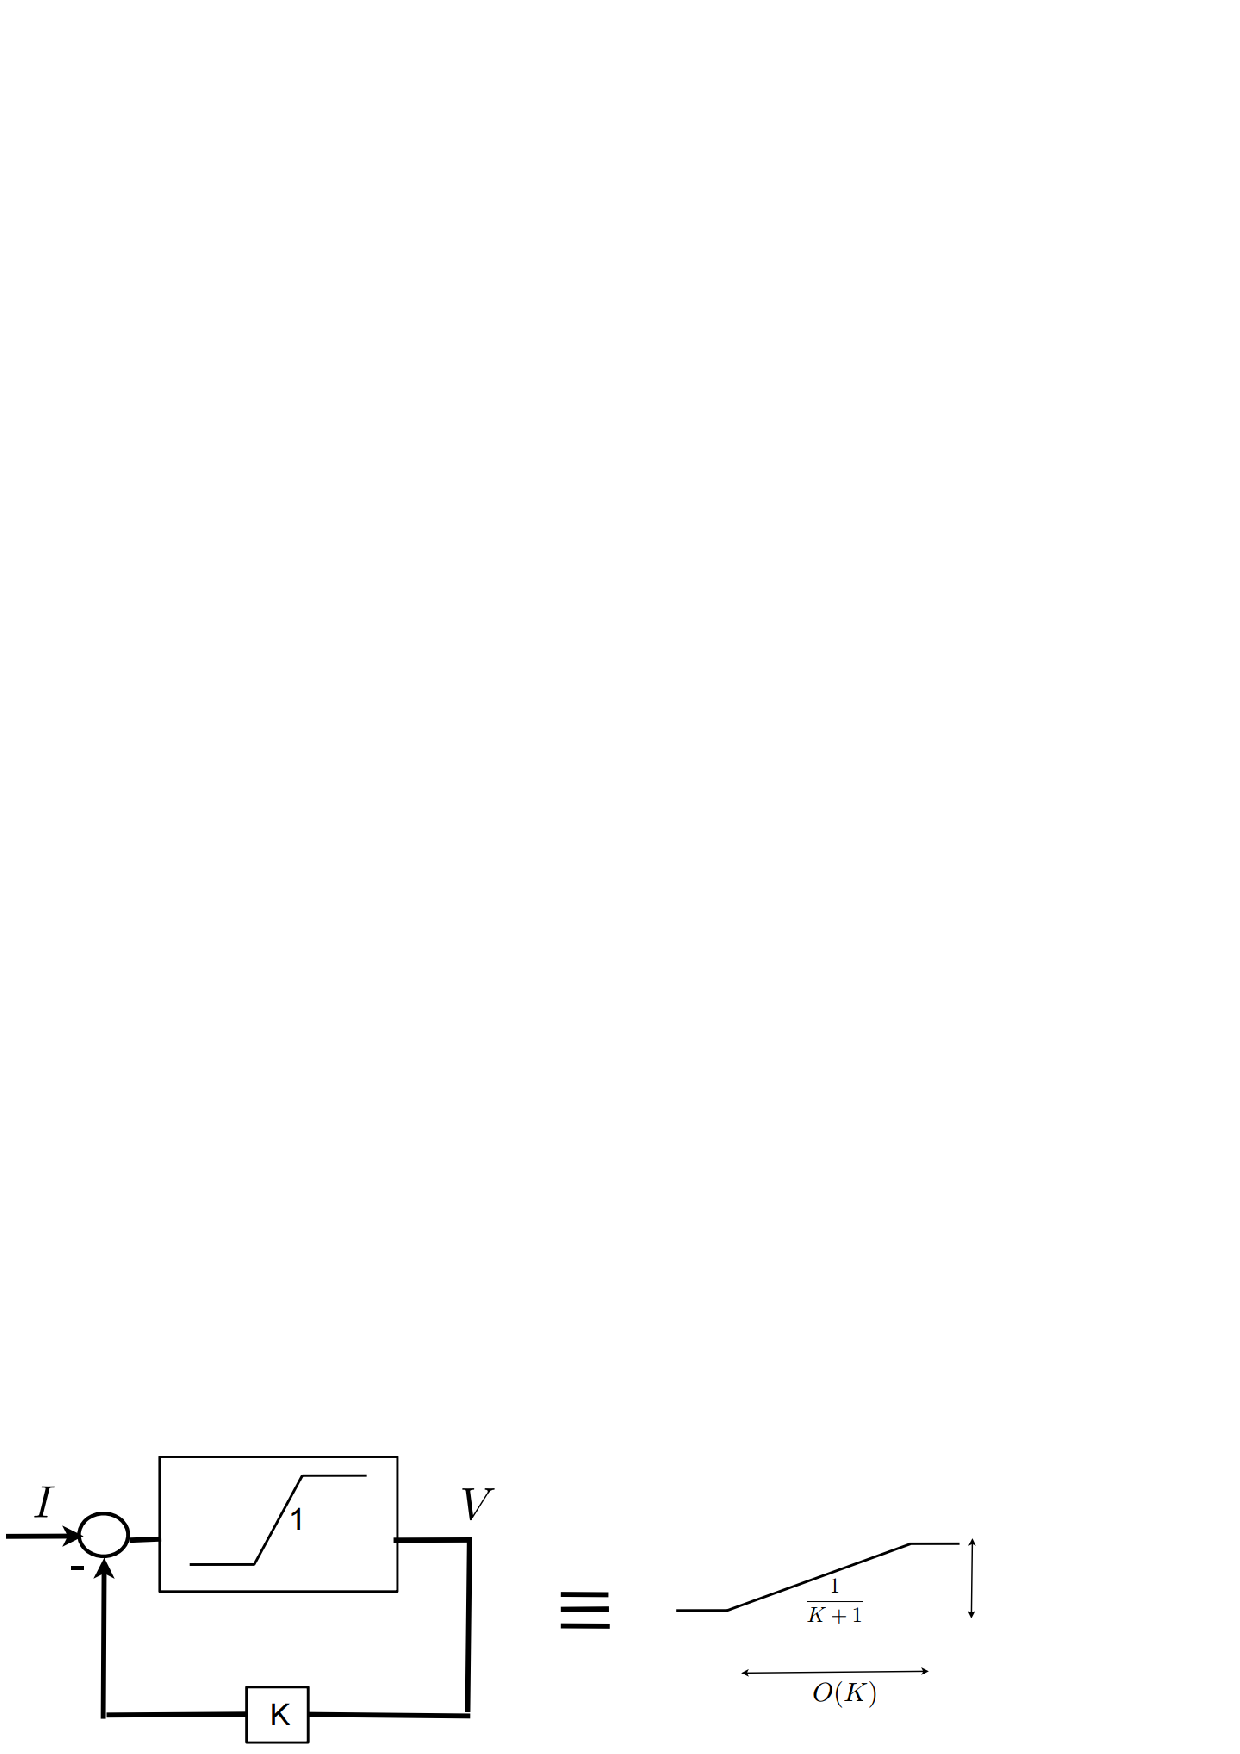
\includegraphics[width=1\linewidth]{black_negative}
\end{figure}
\begin{center}
$V = sat_{1}(I - KV) \equiv V = sat_{\frac{1}{1+K}}(I)$\\
\end{center}
\medskip
Sensitivity domain is spread by negative feedback\\
(The essence of control theory)
\end{frame}

%------------------------------------------------

\begin{frame}
\frametitle{Black principle: positive feedback 'quantizes'}
\begin{figure}
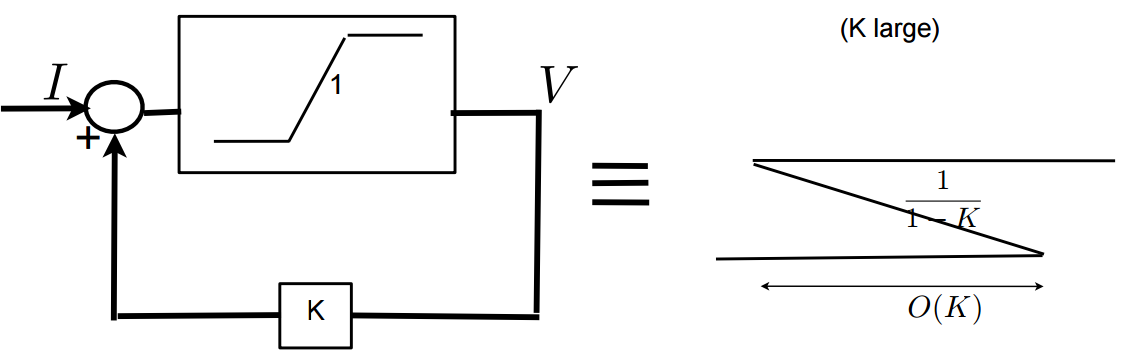
\includegraphics[width=1\linewidth]{black_positive}
\end{figure}
\[   
V =  sat_{1}(I + KV) \equiv V =
     \begin{cases}
       \mbox{+1} &\quad \text{$I \geq -1-K$}\\
       \mbox{-1} &\quad \text{$I \leq K-1$}\
     \end{cases}
\]
Sensitivity domain is spread by negative feedback\\
$\;$
\end{frame}

%------------------------------------------------

\begin{frame}
\frametitle{Black feedback principle}
\vspace{-2ex}
\begin{columns}[c]

\column{.5\textwidth}
\begin{figure}
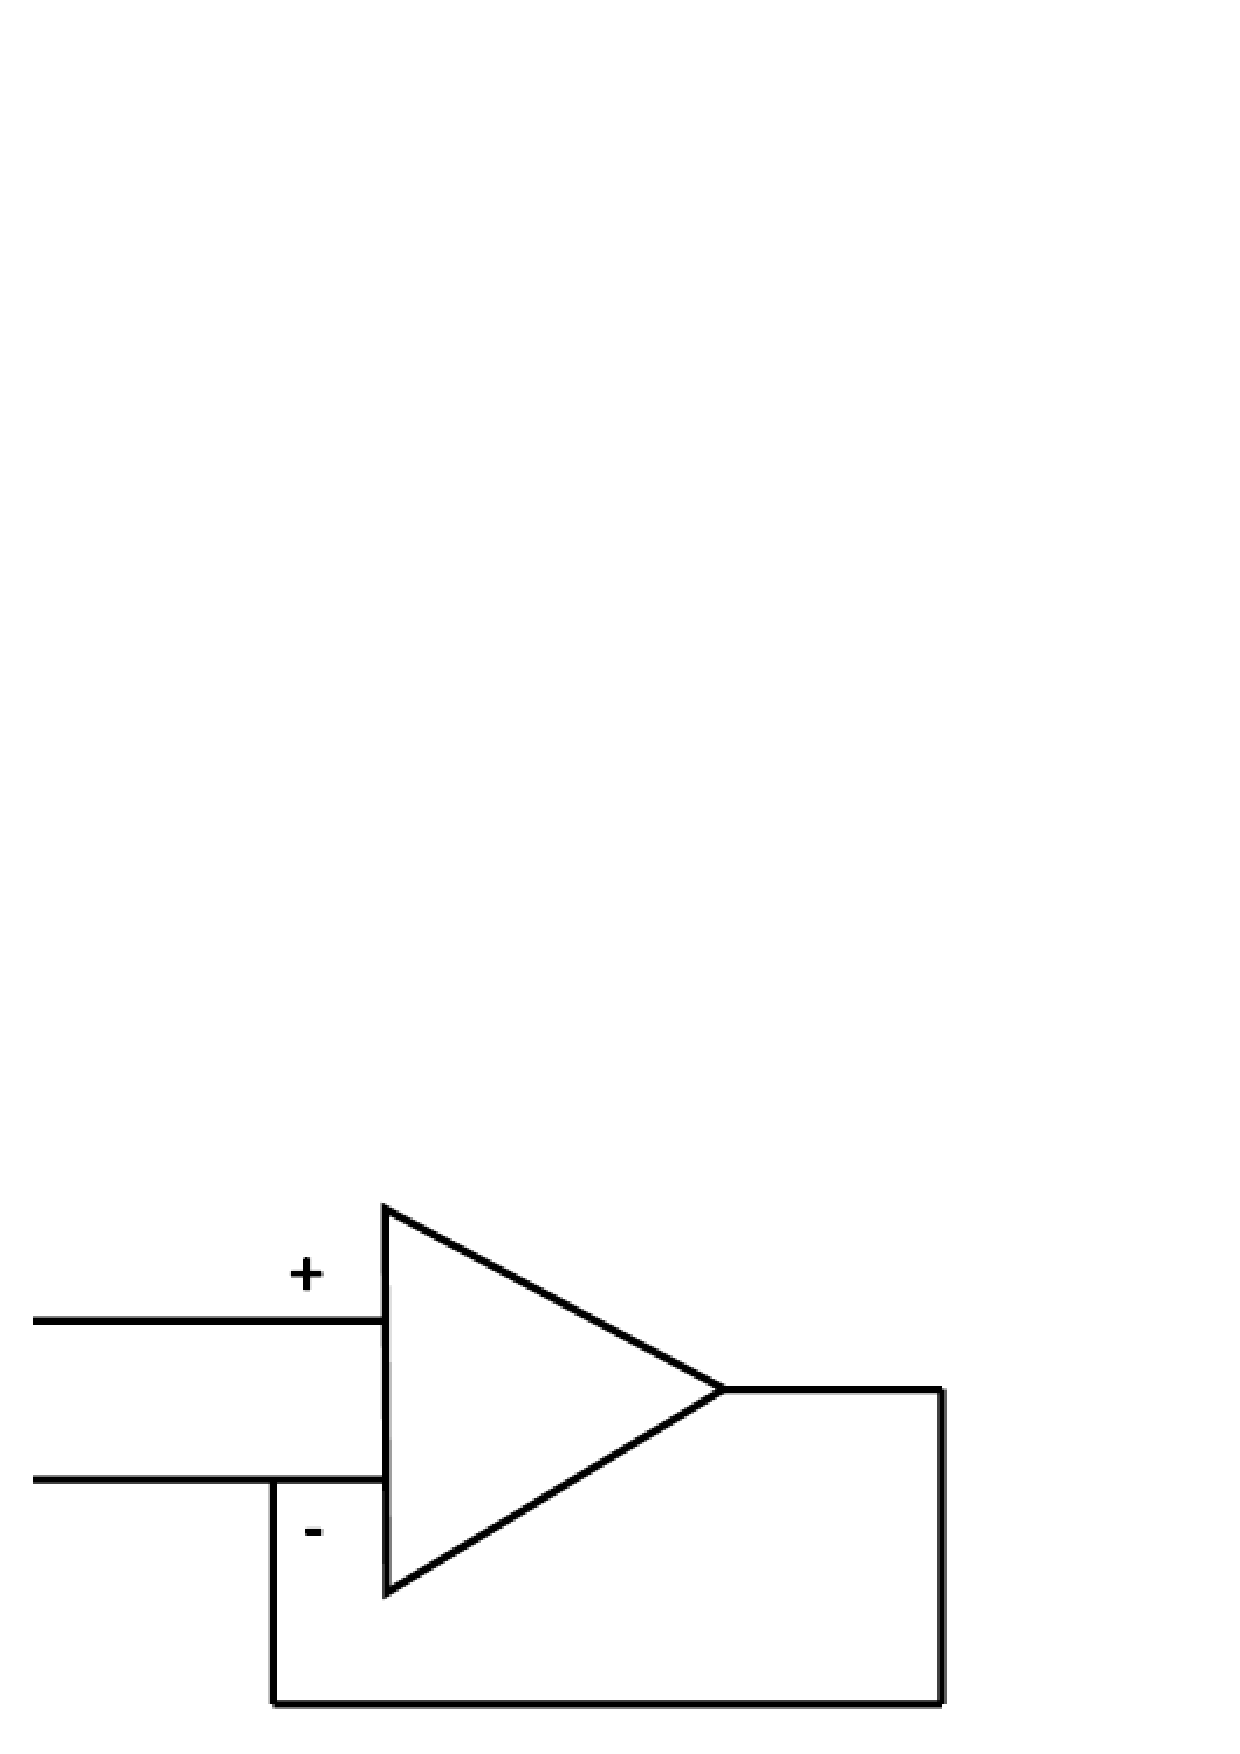
\includegraphics[width=1\linewidth]{negative}
\end{figure}
\vspace{-4ex}
\begin{enumerate}
\item Negative feedback linearizes
\item Continuous behavior
\item Analog technology
\item Output primarily reflects the input
\item Loops enhance or amplify the changes between input and output
\end{enumerate}

\column{.5\textwidth}
\begin{figure}
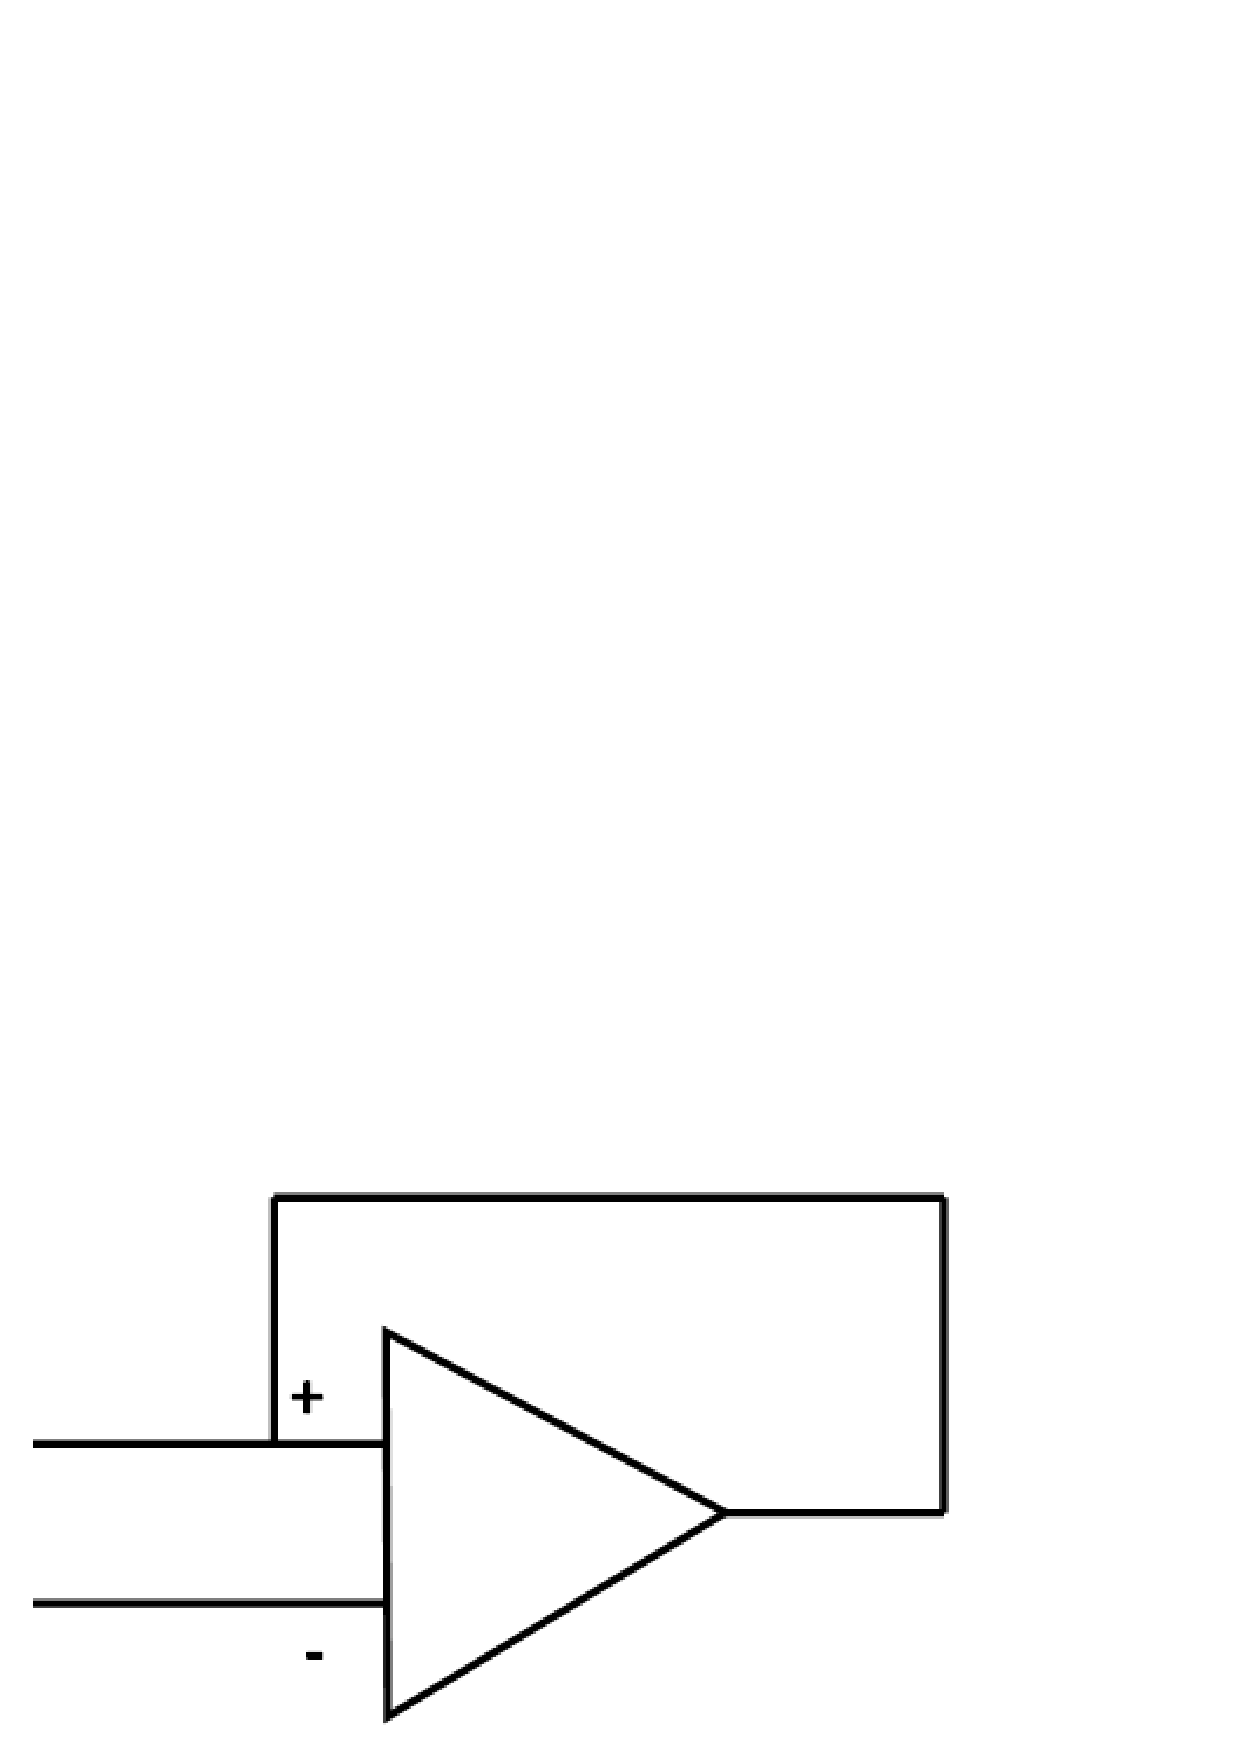
\includegraphics[width=1\linewidth]{positive}
\end{figure}
\vspace{-4ex}
\begin{enumerate}
\item Positive feedback quantizes
\item On-Off behavior
\item Digital Technology
\item Output primarily reflects memory of the past
\item Loops tend to dampen or buffer the changes between input and output
\end{enumerate}

\end{columns}
\end{frame}

%------------------------------------------------

\begin{frame}
\frametitle{Balanced feedback 'localizes'}
\vspace{-2ex}
\begin{columns}[c]

\column{.3\textwidth}
\begin{figure}
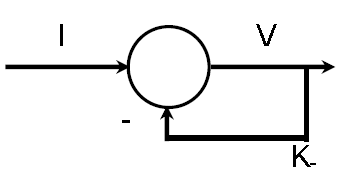
\includegraphics[width=1\linewidth]{linear}
\end{figure}
\center{\textit{\Large{'linear'}}}\\
\center{$|k| large$}

\column{.3\textwidth}
\begin{figure}
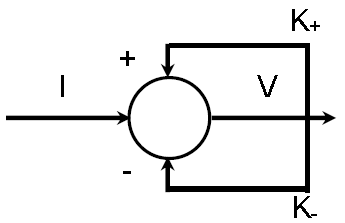
\includegraphics[width=1\linewidth]{localized}
\end{figure}
\vspace{-5ex}
\center{\textit{\Large{'localized'}}}\\
\center{$|k| small$}

\column{.3\textwidth}
\begin{figure}
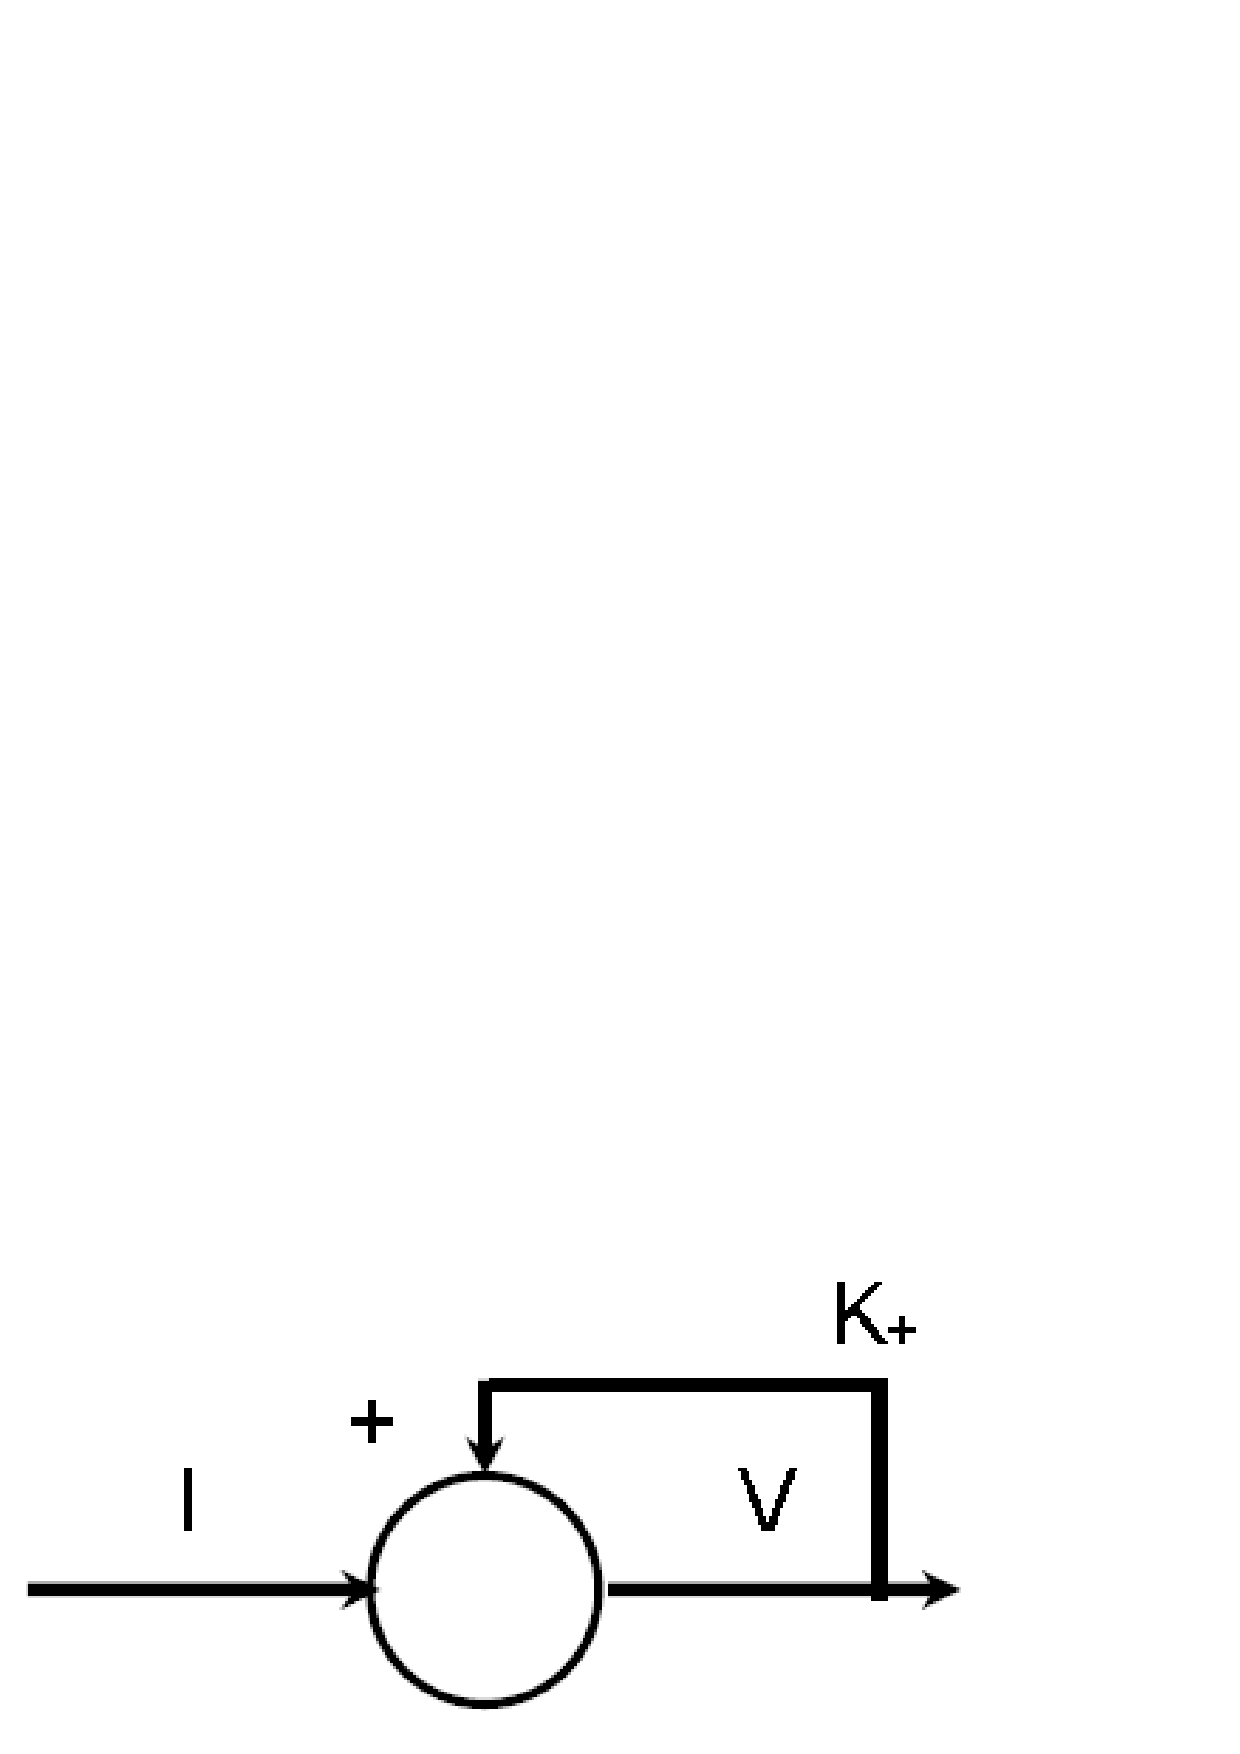
\includegraphics[width=1\linewidth]{memory}
\end{figure}
\center{\textit{\Large{'memory'}}}\\
\center{$|k| large$}

\end{columns}
\begin{figure}
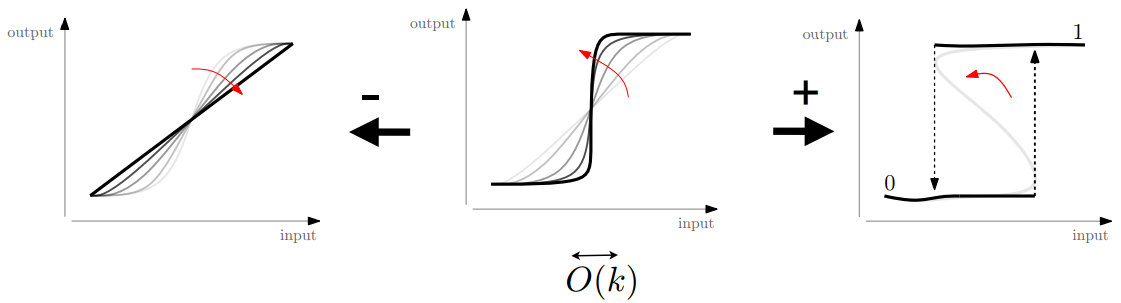
\includegraphics[width=1\linewidth]{balanced_feedback}
\end{figure}
\vspace{-2ex}
\center{$k \approx K_{+} - K_{-}$}
\end{frame}

%------------------------------------------------

\begin{frame}
\frametitle{Robust space + time localization by feedback}
\begin{figure}
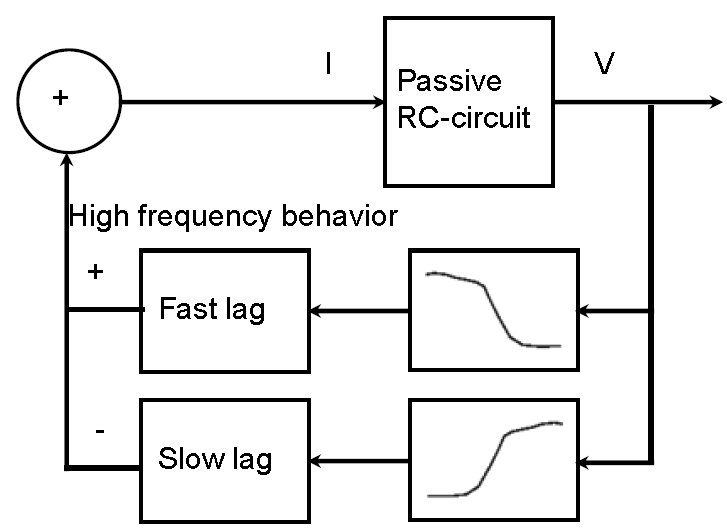
\includegraphics[width=.7\linewidth]{robust}
\end{figure}
Low frequency behavior\\
Necessary localization in same frequency range!
\end{frame}

\end{document}